\usepackage{}\documentclass[oneside]{book}
\usepackage[top=1.5cm, bottom=1.cm, left=1.5cm, right=1.5cm]{geometry}
\usepackage{graphicx}   % IMPORT IMG
\usepackage{hyperref}   % IMPORT URL
\usepackage{minted}     % IMPORT CODE
\usepackage{svg}
\usepackage{caption} 
\usepackage[section]{placeins}

%% -- Front Page -- %%
\usepackage{fancyhdr}
\pagestyle{fancy}
\fancyhf{}
\fancyhead[L]{\leftmark}
\fancyhead[R]{Rapport de projet}
\fancyfoot[C]{\thepage}
\usepackage{titlesec}

%% -- Space Chapter -- %%
\titleformat{\chapter}[display]
{\normalfont\huge\bfseries}{\chaptertitlename\ \thechapter}{20pt}{\Huge}
\titlespacing*{\chapter}{0pt}{0pt}{40pt}

% ------------ BEGIN DOCUMENT
\begin{document}

% ---------------------------- TITRE
\begin{titlepage}
\newcommand{\HRule}{\rule{\linewidth}{0.5mm}} 
\center

% ---------------------------- UNIVERSITE
\textsc{\LARGE Université de Montpellier}\\[0.2cm] 
\textsc{\Large M1 IMAGINE}\\[1.5cm] 

% ---------------------------- TITRE
\HRule \\[0.5cm]
{ \huge \bfseries Rapport TP Analyse et Traitement des Images 1 }\\[0.4cm]
{   HAI804I }\\[0.2cm]
{ \huge \bfseries Rapport TP Codage et compression 1 }\\[0.4cm]
{   HAI809I }\\[0.2cm]
\HRule \\[1.2cm]
 
% ---------------------------- MODULE
\textsc{\large Rapport de TP }\\[0.1cm] 

% ---------------------------- NOMS & ENCADRANT
\begin{minipage}[t]{0.5\textwidth}
    \begin{flushleft}
        \textbf{Étudiant :}\\
        M. Mathieu \textsc{LADEUIL}\\
        \vspace*{0.5cm}

    \end{flushleft}
\end{minipage}%
%
\begin{minipage}[t]{0.5\textwidth}
    \begin{flushright}
        \vspace*{1.8cm}
        \textbf{Année :} 2022\\
    \end{flushright}
\end{minipage}\\[3cm]

\newpage

\end{titlepage}
 \section*{I. Seuillage d'une image au format pgm}
 
On réalise le test du programme de seuillage testgrey.cpp sur l'image 01.pgm avec trois seuils.

\FloatBarrier
\begin{figure}[!htb]
   \begin{minipage}{0.5\textwidth}
     \centering
     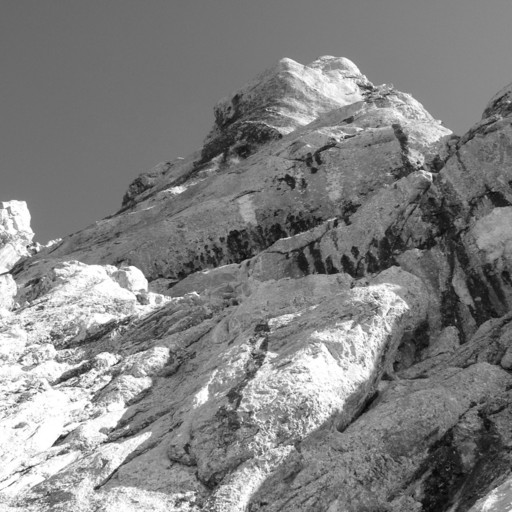
\includegraphics[width=.7\linewidth]{01.jpg}
     \caption{Image originale}
   \end{minipage}\hfill
   \begin{minipage}{0.5\textwidth}
     \centering
     \includegraphics[width=.7\linewidth]{img/.png}
     \caption{Seuil 50}
   \end{minipage}\hfill
   \begin{minipage}{0.5\textwidth}
     \centering
     \includegraphics[width=.7\linewidth]{img/.png}
     \caption{Seuil 100}
   \end{minipage}
   \begin{minipage}{0.5\textwidth}
     \centering
     \includegraphics[width=.7\linewidth]{img/.png}
     \caption{Seuil 200}
   \end{minipage}
\end{figure}
\FloatBarrier

  \end{document}